\section{Pulse detection}
In order to process any pulses they must be first detected. 
The window of interest containing a pulse to be analysed
must be properly distinguished from the surrounding noise.
Although detection is a must, it also brings the added benefit
of data rate reduction. If pulses can be accurately 
marked within a signal it is possible to transfer only
those samples that compose the events to the host PC. 


The ADQ14 is capable of sampling signals with a frequency of
up to 1 GHz. With two bytes per sample, a single channel 
generates 2 GBs of raw data per second. For the PCIe 2.0 interface,
that is used in this work, the manufacturer's 
datasheet specifies a theoretical maximum throughput of 3.2 GB/s.
Even if this perfect limit could be obtained it would not allow 
for two channels to be active at once.
Using pulse detection for data reduction is thus unavoidable.
It is crucial to use a robust algorithm for this process to ensure 
that almost no pulses go unnoticed and near to none
false positives are transmitted.

\subsection{Level trigger}
The most basic approach to detection is a level trigger,
a technology available in virtually any spectroscope. As shown in 
\autoref{fig:level_trigger}, a trigger occurs when
the input signal crosses a predefined voltage level,
either on a rising or a falling edge. The point at which
this happens marks the beginning of a record window.
In the simplest case the end of a window is placed
a fixed duration from the start. Samples within that window
form a region of interest and are transferred further
down the processing pipeline.
\begin{figure}[H]
  \centering
  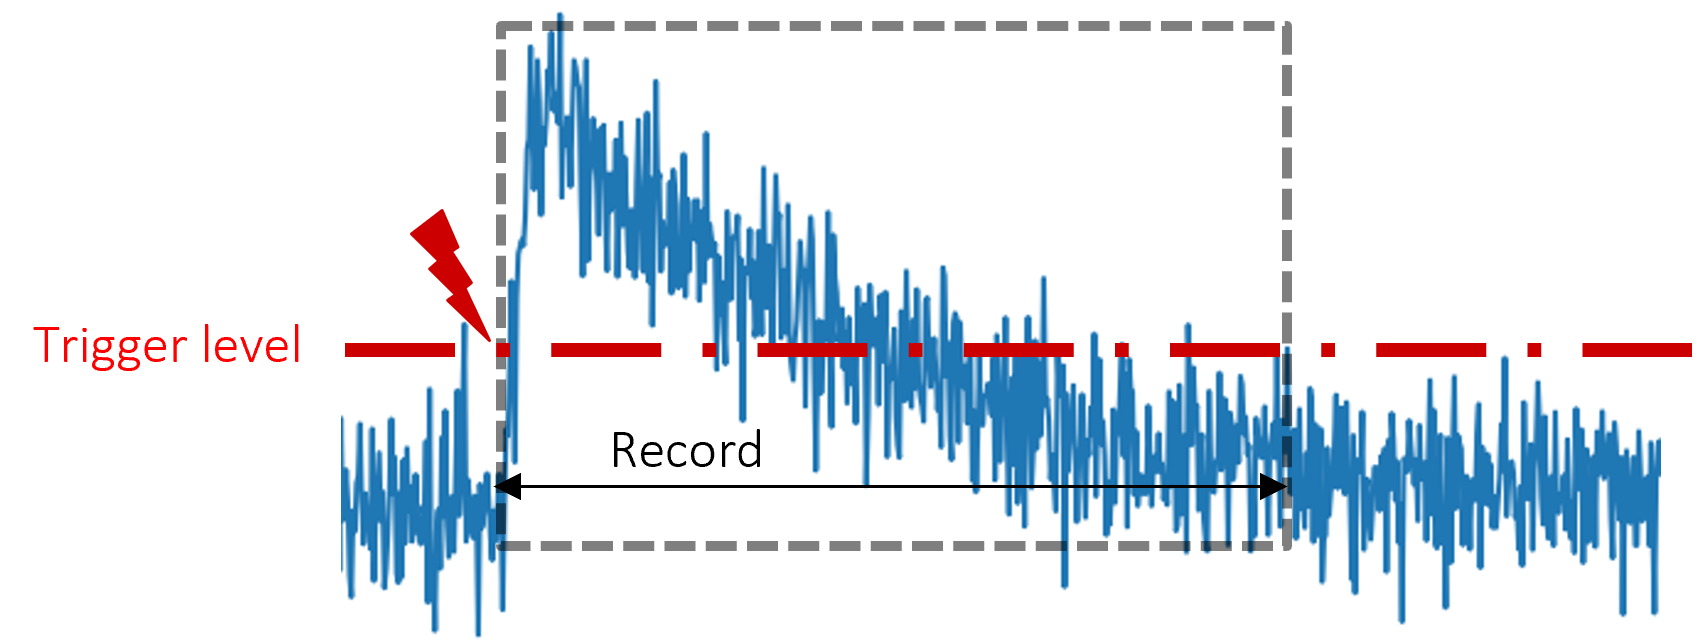
\includegraphics[width=.5\linewidth]{media/level_trigger.png}
  \caption{Level trigger}
  \label{fig:level_trigger}
\end{figure}


Once a window finishes, no more events are detected
until the signal returns to a value below the trigger level
(for rising edge triggering). This reset value might be 
set to be equal to the trigger level, however such approach
might lead to a scenario shown in \autoref{fig:lt_no_hysteresis}.
In a noisy environment the signal might falsely trigger immediately after
a window ends due to a random high spike on the slower falling edge of
an exponential pulse.
\begin{figure}[H]
  \centering
  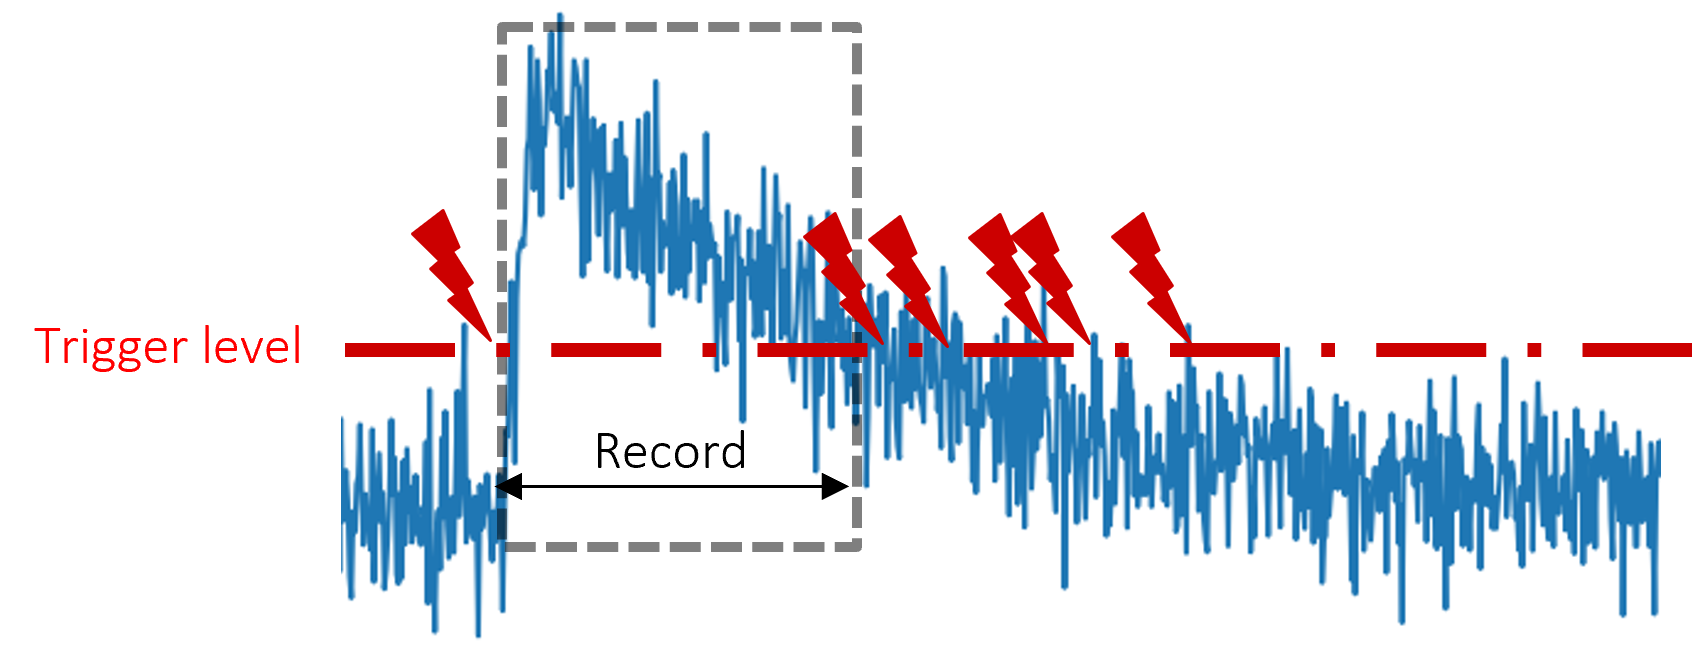
\includegraphics[width=.5\linewidth]{media/lt_no_hysteresis.png}
  \caption{Level trigger with no hysteresis}
  \label{fig:lt_no_hysteresis}
\end{figure}

To prevent such false triggers typically some form of a hysteresis is used.
The reset level is shifted downwards, so that the input signal must cross
such a threshold that the random noise is almost guaranteed to never cause false 
triggers. \autoref{fig:lt_hysteresis} shows a hysteresis mitigating some false triggers.
Some of the false triggers from \autoref{fig:lt_no_hysteresis} are removed, however 
due to the high noise some still persist.
\begin{figure}[H]
  \centering
  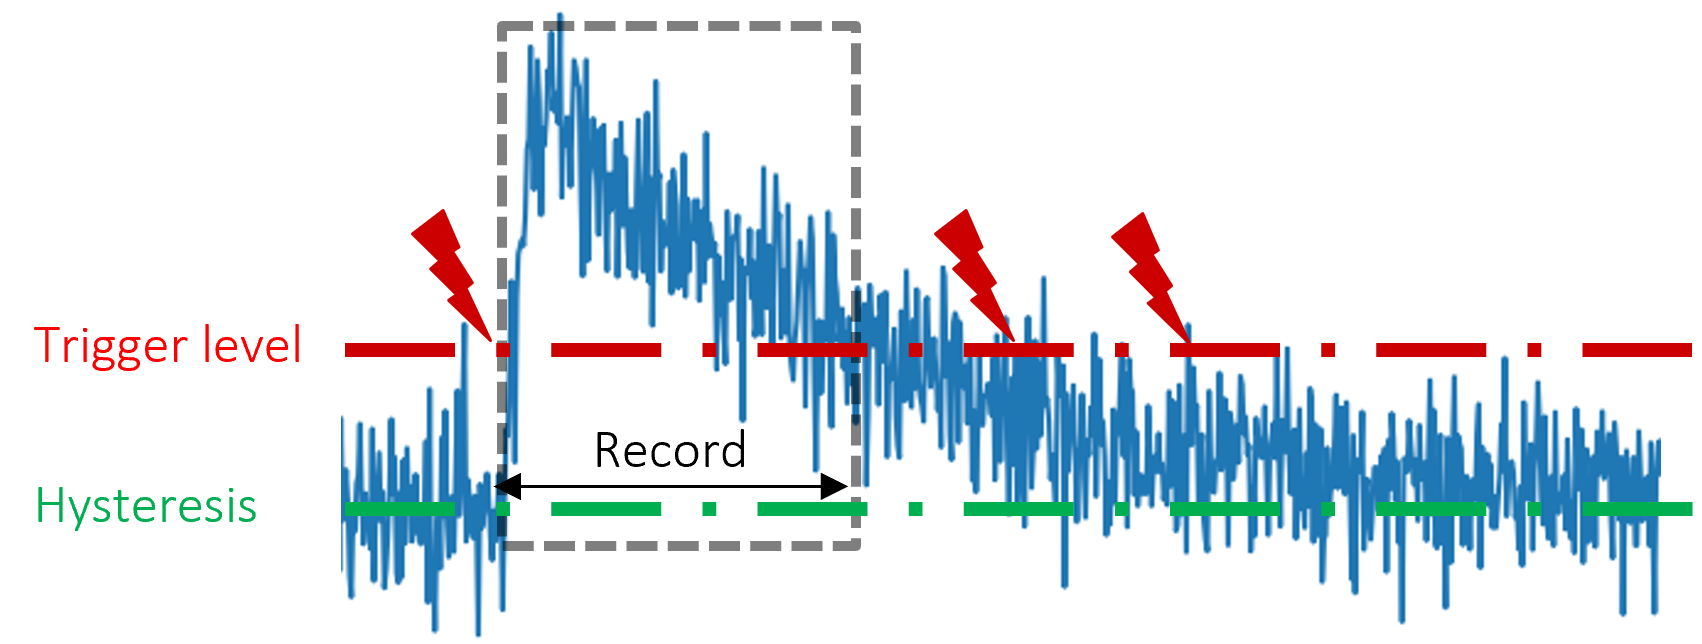
\includegraphics[width=.5\linewidth]{media/lt_hysteresis.png}
  \caption{Level trigger with a hysteresis}
  \label{fig:lt_hysteresis} 
\end{figure}

With the slow falling edge of a pulse care must be taken not to 
overestimate the hysteresis. By setting the reset level too far away
from the trigger level pile-ups can be missed as pointed to in
\autoref{fig:lt_hysteresis_miss}. With a properly set hysteresis
the level trigger offers performance that is sufficient in most applications,
as suggested by its prevalence in modern spectroscopes.
In a tokamak's environment, however, the hysteresis
alone could potentially prove insufficient due to 
electromagnetic and temperature fluctuations having an effect on noise.
\begin{figure}[H]
  \centering
  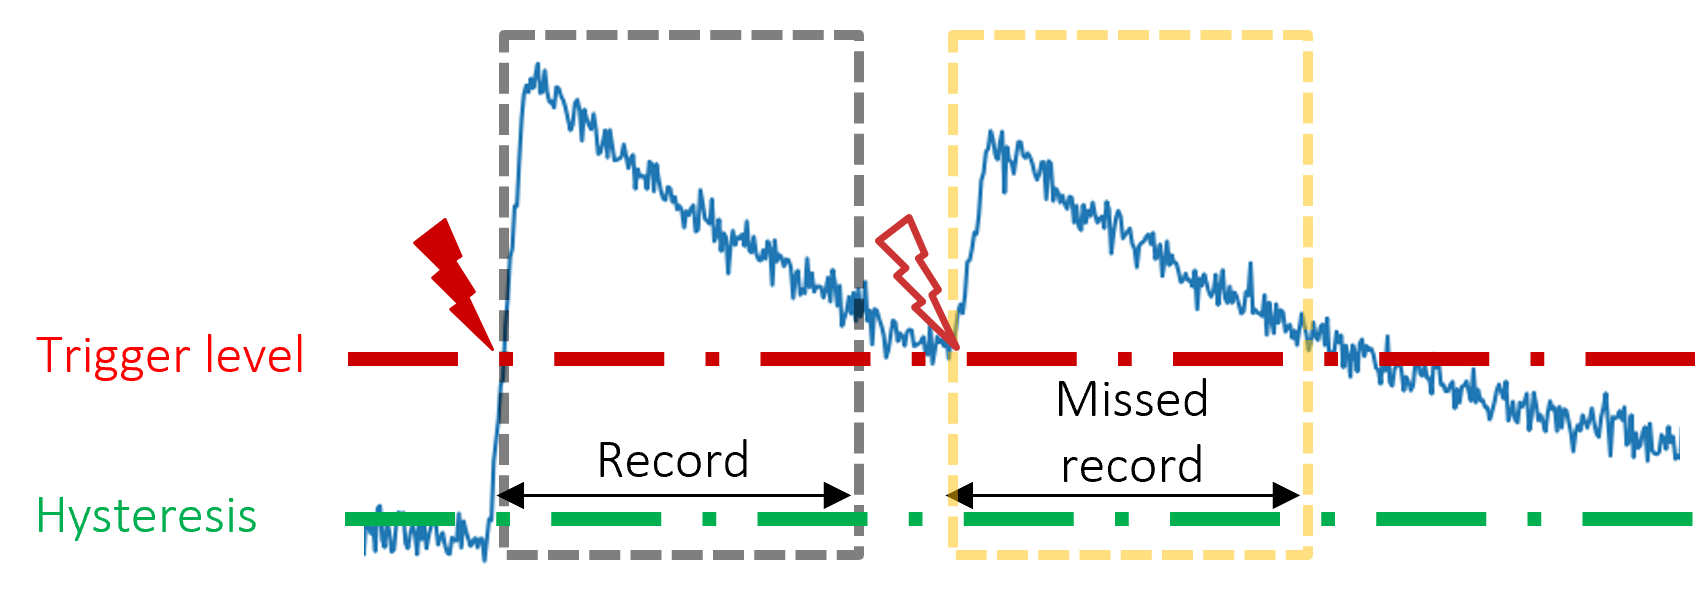
\includegraphics[width=.5\linewidth]{media/lt_hysteresis_miss.png}
  \caption{Level trigger hysteresis causing missed events}
  \label{fig:lt_hysteresis_miss} 
\end{figure}
\subsection{Boxcar filter}

The two problems most apparent to simple level triggering 
are its susceptibility to noise and pulse overlap.
Just as with analogue approaches these two problems 
can be minimized with low-pass and high-pass filtering.
By utilizing a low-pass filter the input signal becomes 
smoother and more averaged, reducing the possibility of 
false triggers caused by random spikes. A high-pass filter
would reduce the DC component of the falling edge of a pulse,
making pile-ups easier to detect.


In the digital domain the simplest filters that perform
these operations are the Moving Average (MA) filter and 
the derivative filter. MA works to reduce the spikes and increase 
SNR. The derivative filter can strip the DC component from
a signal, meaning that the sharp rising edges will become
more attenuated in comparison to the decaying tails.


By combining the concepts of the MA and derivative filters
into a single a Boxcar filter is obtained. An example transfer
function of a Boxcar filter is shown in \autoref{fig:boxcar_transient}.
The effect of the filter on an example exponential pulse are shown 
in \autoref{fig:boxcar_effect}. The filter can be considered
to be a subtraction of two samples averaged with a window
of length $W$ delayed from each other by $W$.



\subsection{Trapezoidal filter}
\subsection{Triangular filter}
\subsection{Other solutions}
\subsection{Simulation performance}
\subsection{Hardware implementation}
\subsubsection{Boxcar filter}
\subsubsection{Trapezoidal filter}
\subsubsection{Triangular filter}
